\title{\textbf{Christian perspectives on sustainability: \\
		The need for numerical answers to philosophical questions.}}
% Sustainability challenges and managing tradeoffs: engineers' need for numerical answers to philosophical questions 
\author{
		% Authors must be italicized.
        \emph{Jeremy Van Antwerp} and \emph{Matthew Kuperus Heun}%
\footnote{
Engineering Department, 
Calvin College,
Grand Rapids, MI, 49546, USA}
}

\documentclass[12pt]{article}

% CEC papers should be set in Times New Roman.
% https://tex.stackexchange.com/questions/153168/how-to-set-document-font-to-times-new-roman-by-command
% suggests the following.
\usepackage{mathptmx}             % For Times New Roman font (or a close approximation thereof).
\usepackage[margin=1in]{geometry} % For 1-inch margins all around.
\usepackage[document]{ragged2e}   % For left justification.
\usepackage{parskip}              % For double-spacing between paragraphs.
\usepackage{nopageno}             % To eliminate page numbers.
% For MLA bibliography. See https://www.ctan.org/pkg/biblatex-mla?lang=en for details.
\usepackage[american]{babel}
\usepackage{csquotes}
\usepackage[style=mla-new]{biblatex}
\addbibresource{JVAMKH.bib}

\usepackage{titlesec}             % To change formats of section titles, etc.
\titleformat*{\section}{\normalsize}
\titleformat*{\subsection}{\normalsize}
\titleformat*{\subsubsection}{\normalsize}
\titleformat*{\paragraph}{\itshape} % Set paragraph titles to italics
\usepackage{abstract}             % Set characteristics of the abstract
\setlength{\absleftindent}{0in}   % Do not indent left side
\setlength{\absrightindent}{0in}  % Do not indent right side
\usepackage{url}
\setlength{\parindent}{0in}       % Do not indent the 1st line of paragraphs.
\setlength{\parskip}{12pt}        % Instead, add space between paragraphs.
\renewcommand{\abstractnamefont}{\normalfont\normalsize} % Unbold and regular size
\renewcommand{\abstracttextfont}{\normalfont\normalsize} % Unbold and regular size
\date{}                           % To eliminate the date in the title

% To include graphics
\usepackage{graphicx}

% Commands for editing.

\usepackage{xcolor}            % For colored text
\usepackage[normalem]{ulem}    % For \sout command (strikethrough)

% From https://tex.stackexchange.com/questions/130623/crossing-out-using-different-colour,
% Change the \sout color to red
\newcommand{\redsout}{\bgroup\markoverwith{\textcolor{red}{\rule[0.5ex]{2pt}{0.4pt}}}\ULon}

% Use these versions to display changes.
\newcommand{\del}[1]{\textcolor{gray}{\redsout{#1}}}
\newcommand{\ins}[1]{\textcolor{red}{#1}}
\newcommand{\rev}[2]{\del{#1}\ins{#2}}

% Use these versions for a clean copy.
% \newcommand{\del}[1]{}
% \newcommand{\ins}[1]{#1}
% \newcommand{\rev}[2]{#2}



\begin{document}
	
\maketitle

\begin{abstract}
\noindent
\ins{rewrite abstract from scratch. Later.}

\end{abstract}


%%%%%%%%%%%%%%%%%%%%%%%%%%%%%%%%%%%%%%%%%%%%%%%%%%%%%%%%%%%%%%
\section{Sustainability and the disciplines}
\label{sec:sustainability_and_the_disciplines}
%%%%%%%%%%%%%%%%%%%%%%%%%%%%%%%%%%%%%%%%%%%%%%%%%%%%%%%%%%%%%%

Because of circumstances in our world today, 
concerns about environmental, economic, and social 
issues are significant. 
The concept of ``sustainability'' encompasses all three areas
with a view toward the future. 
(See Figure~\ref{fig:3_sustain}.)
One definition of sustainability is
``Sustainability emerges from choices that, on balance, 
promote economic vitality, social equity, and a flourishing natural environment 
both now and for generations to come''~\autocite{Calvin-College-2017}.

Sustainability is considered to be a ``grand challenge,'' 
and becoming more sustainable requires solving 
complex, multidisciplinary, and multifaceted problems
with both technical and non-technical, even philosophical, aspects. 
We engineers design and operate the machines and systems that
generate economic growth by providing employment and economic output, 
enhance society bring people together through communication technologies, and
enhance the natural environment.
But we also design machines and systems that
replace human workers, 
foster online hate, 
and  
consume non-renewable materials
emit pollution, contributing to environmental degradation.
Thus, we have an important role to play in the transition to a sustainable future. 

But what guides engineers to make choices that lead to sustainability?

\begin{figure}
\centering
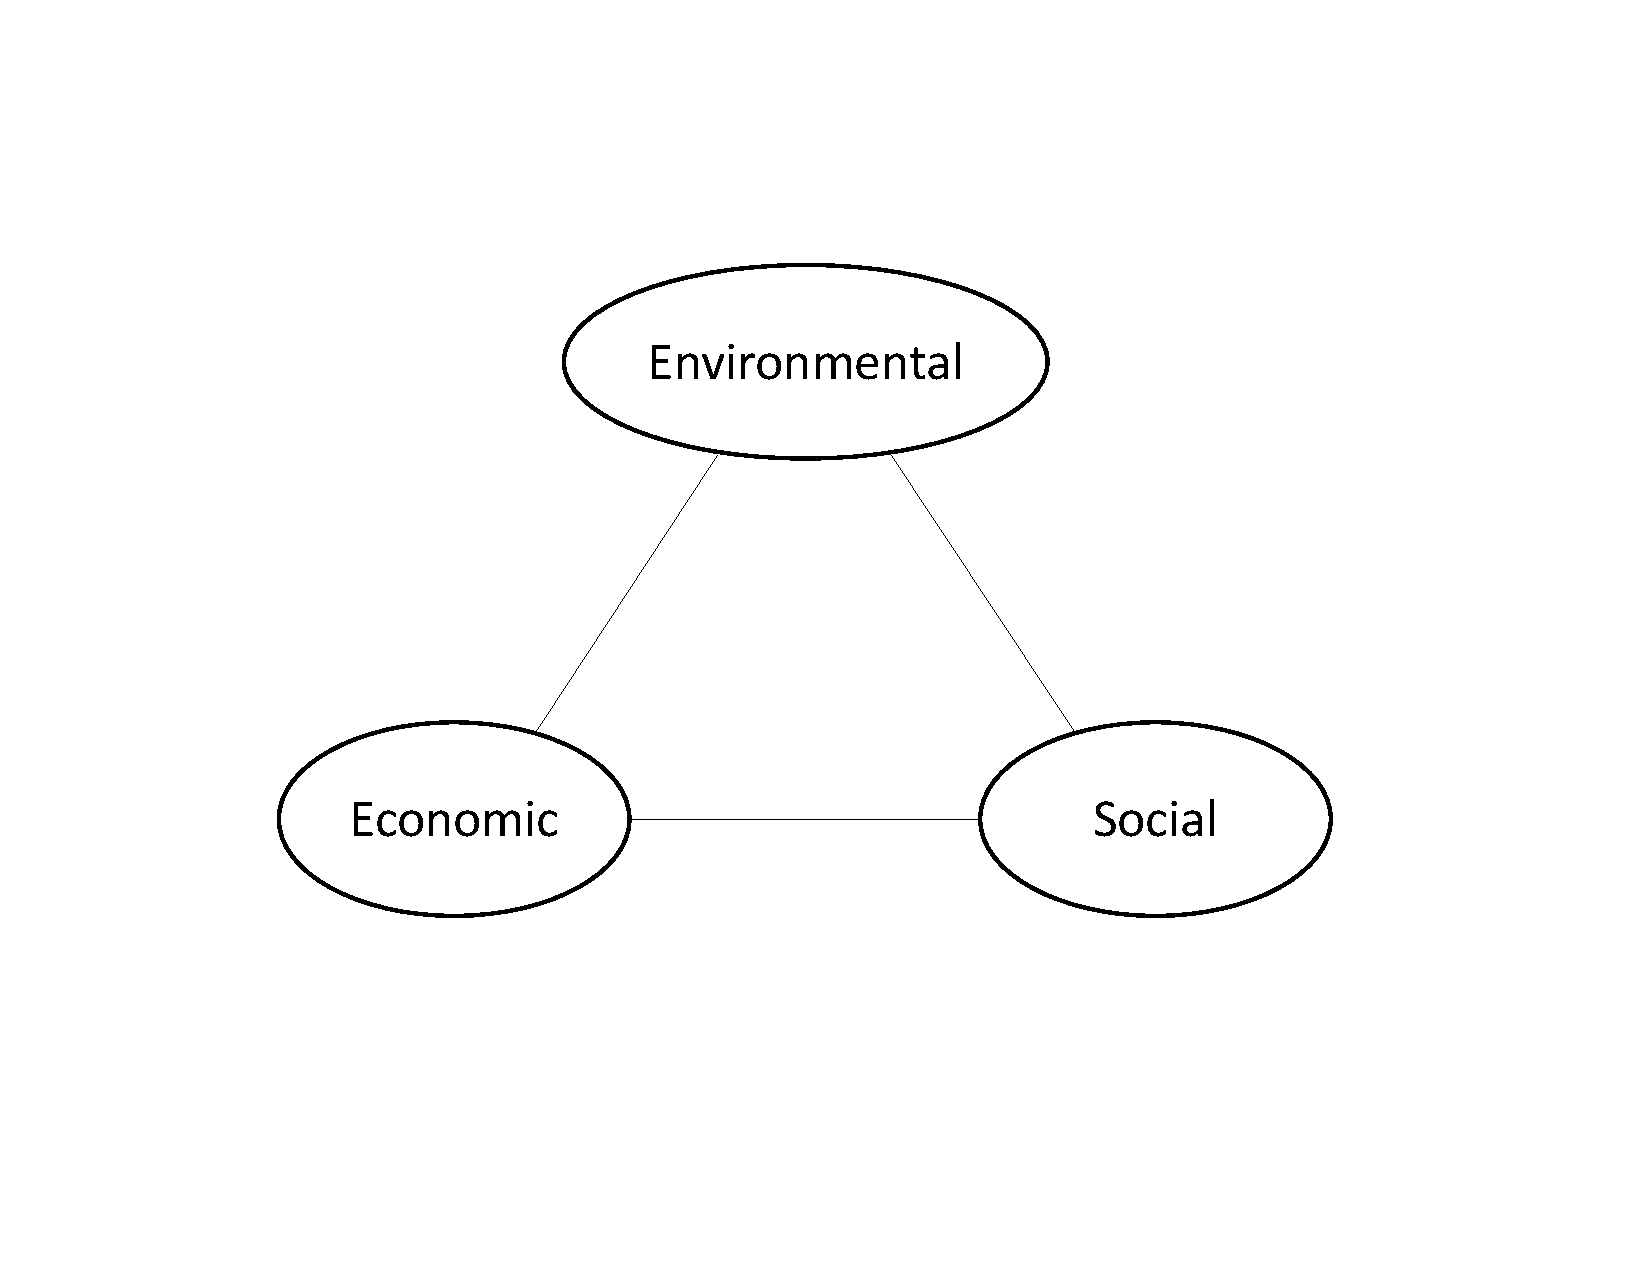
\includegraphics[width=1\linewidth]{figure_other/TriangleDiagram.pdf}
\caption{Three aspects of sustainability.}
\label{fig:3_sustain}
\end{figure}


%%%%%%%%%%%%%%%%%%%%%%%%%%%%%%%%%%%%%%%%%%%%%%%%%%%%%%%%%%%%%%
\section{Questions}
\label{sec:questions}
%%%%%%%%%%%%%%%%%%%%%%%%%%%%%%%%%%%%%%%%%%%%%%%%%%%%%%%%%%%%%%



%%%%%%%%%%%%%%%%%%%%%%%%%%%%%%%%%%%%%%%%%%%%%%%%%%%%%%%%%%%%%%
\section{The need for a theology of sustainability}
\label{sec:need_for_theology_of_sustainability}
%%%%%%%%%%%%%%%%%%%%%%%%%%%%%%%%%%%%%%%%%%%%%%%%%%%%%%%%%%%%%%



%%%%%%%%%%%%%%%%%%%%%%%%%%%%%%%%%%%%%%%%%%%%%%%%%%%%%%%%%%%%%%
\section{Worldviews}
\label{sec:worldviews}
%%%%%%%%%%%%%%%%%%%%%%%%%%%%%%%%%%%%%%%%%%%%%%%%%%%%%%%%%%%%%%


%%%%%%%%%%%%%%%%%%%%%%%%%%%%%%%%%%%%%%%%%%%%%%%%%%%%%%%%%%%%%%
\section{Conclusions}
\label{sec:conclusions}
%%%%%%%%%%%%%%%%%%%%%%%%%%%%%%%%%%%%%%%%%%%%%%%%%%%%%%%%%%%%%%



\printbibliography
\end{document}